In this chapter we discuss the results of our MD simulations. Here we start by a scaling performance benchmark in section \ref{sec:md_benchmark} before we in section \ref{sec:md_cylinder_result} move on to a validation of the Knudsen correction we confirmed with the DSMC model. Most of the concepts are equivalent as in DSMC in section \ref{sec:dsmc_parallelization_performance}, so the reader is is assumed to have read that section.

\section{Parallelization performance}
\label{sec:md_benchmark}
The parallelization scheme we have used in MD is very similar to the one we used in DSMC. In section \ref{sec:dsmc_parallelization_performance}, we measured both the strong and the weak scaling efficiency ($\eta_s$ and $\eta_w$) which measure two different ways of scaling the program. We will not repeat the discussion about these except present the result for both scaling for the MD program. 

\subsection{Strong scaling}
The strong scaling efficiency $\eta_s$ tells us how well the program scales if we keep the system size constant while increasing the number of processors. The strong scaling efficiency was defined as
\begin{align}
	\eta_s = \frac{t_1}{Nt_N},
\end{align}
where $t_1$ is the total run time using one processor and $t_N$ is the total run time using $N$ processors. In this benchmark, we chose a system consisting of $48\times48\times48=110592$ unit cells which gives a total of 442368 atoms. When we increase the number of processors, these 48 unit cells per dimension are distributed on the processors. The timestep was $\Delta t = 0.02$ and the initial temperature was approximately $T_0=$\unit{100}{\kelvin} so that the final gas temperature was around $T=$\unit{60}{\kelvin}. This fall in temperature is explained by the fact that the FCC lattice is the potential minimum, so with a non-zero temperature, some of the initial kinetic energy will be converted to potential energy. We run the program with the number of processors in the range 1 to 512. In table \ref{tab:md_strong_scaling} we have presented the results for this benchmark which is summarized in figure \ref{fig:md_strong_scaling}. We see that when going from one to two processors, we get a more than ideal speedup with $\eta_s(N_\text{CPU}=2)=1.17$ which can be explained by the CPU cache. When a processor compute with a value stored at some memory address, it will first look in the three levels of cache to see if the value of the memory address is cached there. Cached values are much faster available for computation than those only in the memory. When going from one processor to two, a larger part of the positions array (which is used in the force calculation) can be cached, hence a more than double speedup is obtainable. When using a larger number of processors, the MPI communication time starts increasing so that the total time increases per cpu. 

\begin{table}[h]
\begin{center}
    \begin{tabular}{|l|l|l|l|l|}
    \hline
    $N_\text{CPU}$ & $N_\text{atoms}/N_\text{CPU}$ & $t_N$ & $\eta_s$ \\ \hline
    1 & 442368 & \unit{29196}{\second} & 1.00\\
    \hline
    2 & 221184 & \unit{12471}{\second} & 1.17\\
    \hline
    4 & 110592 & \unit{6435}{\second} & 1.13\\
    \hline
    8 & 55296 & \unit{3469}{\second} & 1.05\\
    \hline
    16 & 27648 & \unit{1926}{\second} & 0.95\\
    \hline
    32 & 13824 & \unit{1021}{\second} & 0.89\\
    \hline
    64 & 6912 & \unit{715}{\second} & 0.64\\
    \hline
    128 & 3456 & \unit{375}{\second} & 0.61\\
    \hline
    256 & 1728 & \unit{220}{\second} & 0.52\\
    \hline
    512 & 864 & \unit{150}{\second} & 0.38\\
    \hline
    \end{tabular}
    \caption{Benchmark results showing the strong scaling efficiency $\eta_s$ for the MD program. We see that when going from one to two processors, we get a more than ideal speedup with $\eta_s(N_\text{CPU}=2)=1.17$ which can be explained by the CPU cache. When a processor compute with a value stored at some memory address, it will first look in the three levels of cache to see if the value of the memory address is cached there. Cached values are much faster available for computation than those only in the memory. When going from one processor to two, a larger part of the positions array (which is used in the force calculation) can be cached, hence a more than double speedup is obtainable. When using a larger number of processors, the MPI communication time starts increasing so that the total time increases per cpu.}
    \label{tab:md_strong_scaling}
    \end{center}
\end{table}

\begin{figure}[h!]
\begin{center}
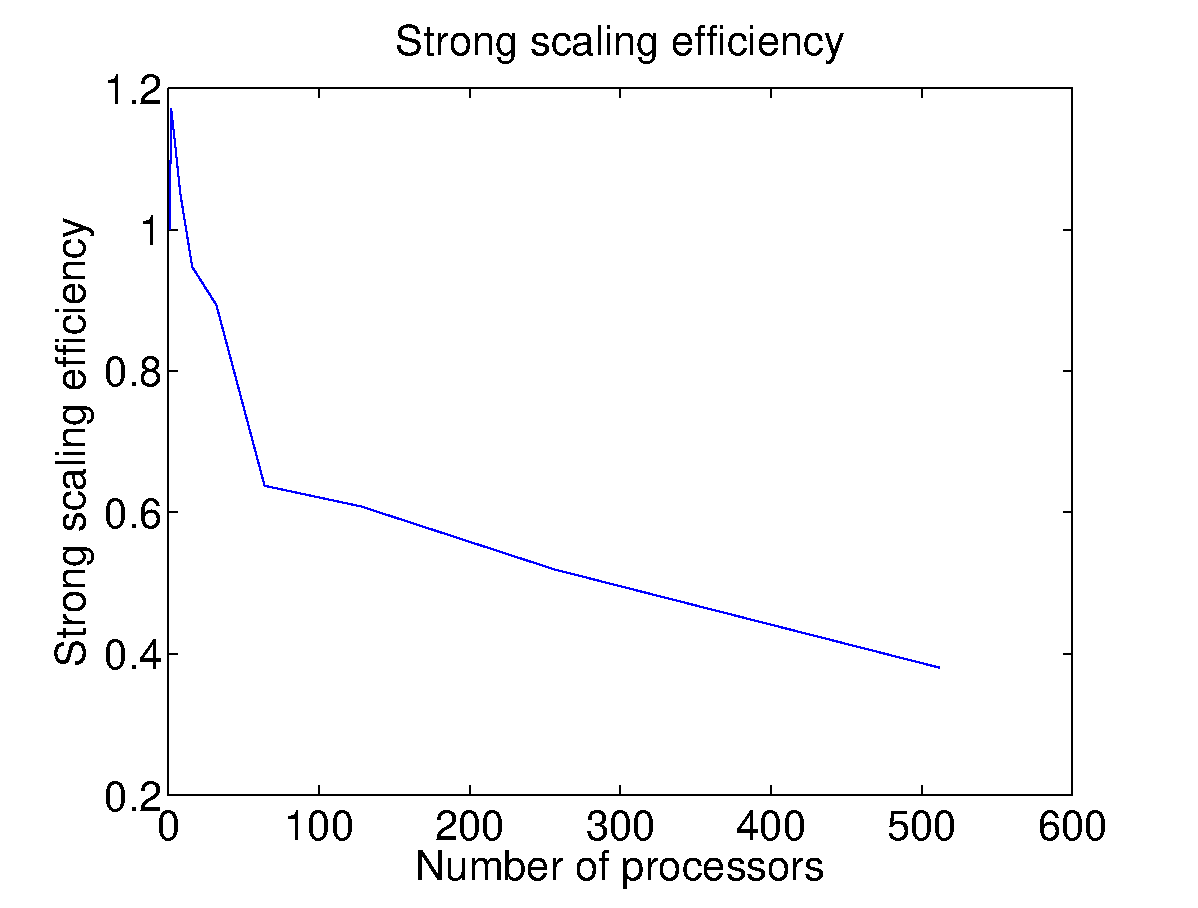
\includegraphics[width=0.7\textwidth, trim=0cm 0cm 0cm 0cm, clip]{MD/figures/strong_scaling.eps}
\end{center}
\caption{Benchmark results showing the strong scaling efficiency $\eta_s$ for the MD program. We see that when going from one to two processors, we get a more than ideal speedup with $\eta_s(N_\text{CPU}=2)=1.17$ which can be explained by the CPU cache. When a processor compute with a value stored at some memory address, it will first look in the three levels of cache to see if the value of the memory address is cached there. Cached values are much faster available for computation than those only in the memory. When going from one processor to two, a larger part of the positions array (which is used in the force calculation) can be cached, hence a more than double speedup is obtainable. When using a larger number of processors, the MPI communication time starts increasing so that the total time increases per cpu.}
\label{fig:md_strong_scaling}
\end{figure}

\subsection{Weak scaling}
If we increase the number of processors, but keep the nubmer of atoms per processor constant, we can use the weak scaling efficiency $\eta_w$ to see how the program scales in this case. The weak scaling efficiency is defined as
\begin{align}
	\eta_w = \frac{t_1}{t_N},
\end{align}
where again $t_1$ is the total run time using one processor and $t_N$ is the run time using $N$ processors. In this benchmark, we chose $10\times10\times10=1000$ unit cells per processor yielding a total of 4000 atoms per cpu. The timestep here as well is $\Delta t = 0.02$ with the same initial temperature as in the strong scaling so that the final temperature is approximately $T=$\unit{60}{\kelvin}. In table \ref{tab:md_weak_scaling} and figure \ref{fig:md_weak_scaling}, we have presented the results for the weak scaling. 

\begin{table}[h]
\begin{center}
    \begin{tabular}{|l|l|l|l|l|}
    \hline
    $N_\text{CPU}$ & $N_\text{atoms}$ & $t_N$ & $\eta_w$ \\ \hline
    1 & 4000 & \unit{1246}{\second} & 1.00\\
    \hline
    2 & 8000 & \unit{1278}{\second} & 0.97\\
    \hline
    4 & 16000 & \unit{1398}{\second} & 0.89\\
    \hline
    8 & 32000 & \unit{1441}{\second} & 0.86\\
    \hline
    16 & 64000 & \unit{1521}{\second} & 0.82\\
    \hline
    32 & 128000 & \unit{1620}{\second} & 0.77\\
    \hline
    64 & 256000 & \unit{1639}{\second} & 0.76\\
    \hline
    128 & 512000 & \unit{1735}{\second} & 0.72\\
    \hline
    256 & 1024000 & \unit{2027}{\second} & 0.61\\
    \hline
    512 & 2048000 & \unit{3379}{\second} & 0.37\\
    \hline
    \end{tabular}
    \caption{Benchmark results showing the weak scaling efficiency $\eta_w$ for the MD program. }
    \label{tab:md_weak_scaling}
    \end{center}
\end{table}

\begin{figure}[h!]
\begin{center}
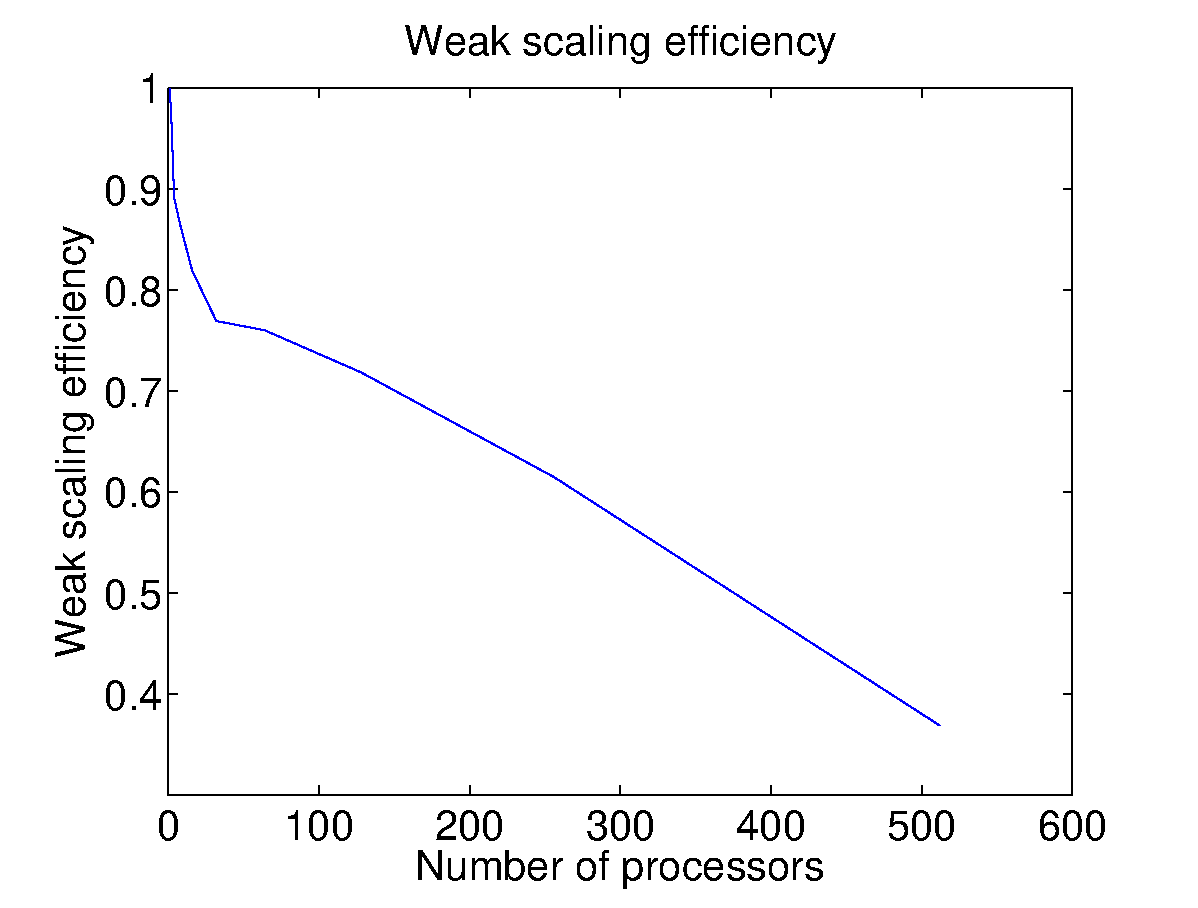
\includegraphics[width=0.7\textwidth, trim=0cm 0cm 0cm 0cm, clip]{MD/figures/weak_scaling.eps}
\end{center}
\caption{Benchmark results showing the weak scaling efficiency $\eta_w$ for the MD program.}
\label{fig:md_weak_scaling}
\end{figure}

\section{Flow in a cylinder, varying Knudsen number}
\label{sec:md_cylinder_result}
We have used the MD program to simulate flow in a cylinder with a fixed radius $R$, just like we did in section \ref{sec:results_for_simple_geometries} with DSMC. We will measure the permeability to see how well the Knudsen correction factor (see section \ref{sec:knudsen_correction}) predicts the permeability for very small pores (here a cylinder) with an atomic model. The cylinder was created with the solid model we described in section \ref{sec:md_simple_model_of_a_solid}. Since the solid now consists of atoms (in DSMC it was just a scalar field defining the surface), we should create the cylinder carefully. We have prepared the system with the following steps
\begin{itemize}
	\item Heat the system 2000 timesteps, $T=$\unit{300}{\kelvin}
	\item Thermalize the system 2000 timesteps
	\item Heat the system 2000 timesteps, $T=$\unit{300}{\kelvin}
	\item Thermalize the system 2000 timesteps
	\item Create cylinder (explained below)
	\item Reduce density (explained below).
\end{itemize}
By first heating the system, we let the system melt from a solid state to a liquid state. This allows the system to become more random than in the initial lattice. Once we create the cylinder, we apply a harmonic oscillator potential on the atoms in the cylinder so they more or less stay in their initial position. We have here chosen a system consisting of $64\times64\times64=262144$ unit cells which gives a total of 1048576 atoms to begin with. This in turn yields a system with size $L_i=336.64Å$ in the $i$th dimension. By choosing the cylinder radius to be $r=0.45L_i$ and the flow in the $z$-direction, we mark all atoms within a distance $r$ from the center (in the $xy$-plane) as gas atoms, and atoms outside $r$ as solid atoms. But the cut-off radius was chosen to be $r_\text{cut}=2.5\sigma$ (see section \ref{sec:md_implementation_two_body_forces}), so the gas atoms inside the cylinder will not feel the precense of the atoms outside $r+2.5\sigma$ directly. To save computation time, we have removed all atoms outside this radius. Such a cylinder is shown in figure \ref{fig:md_cylinder} where the yellow atoms are the solid wall wheras the green atoms are the gas.
\begin{figure}[h!]
\begin{center}
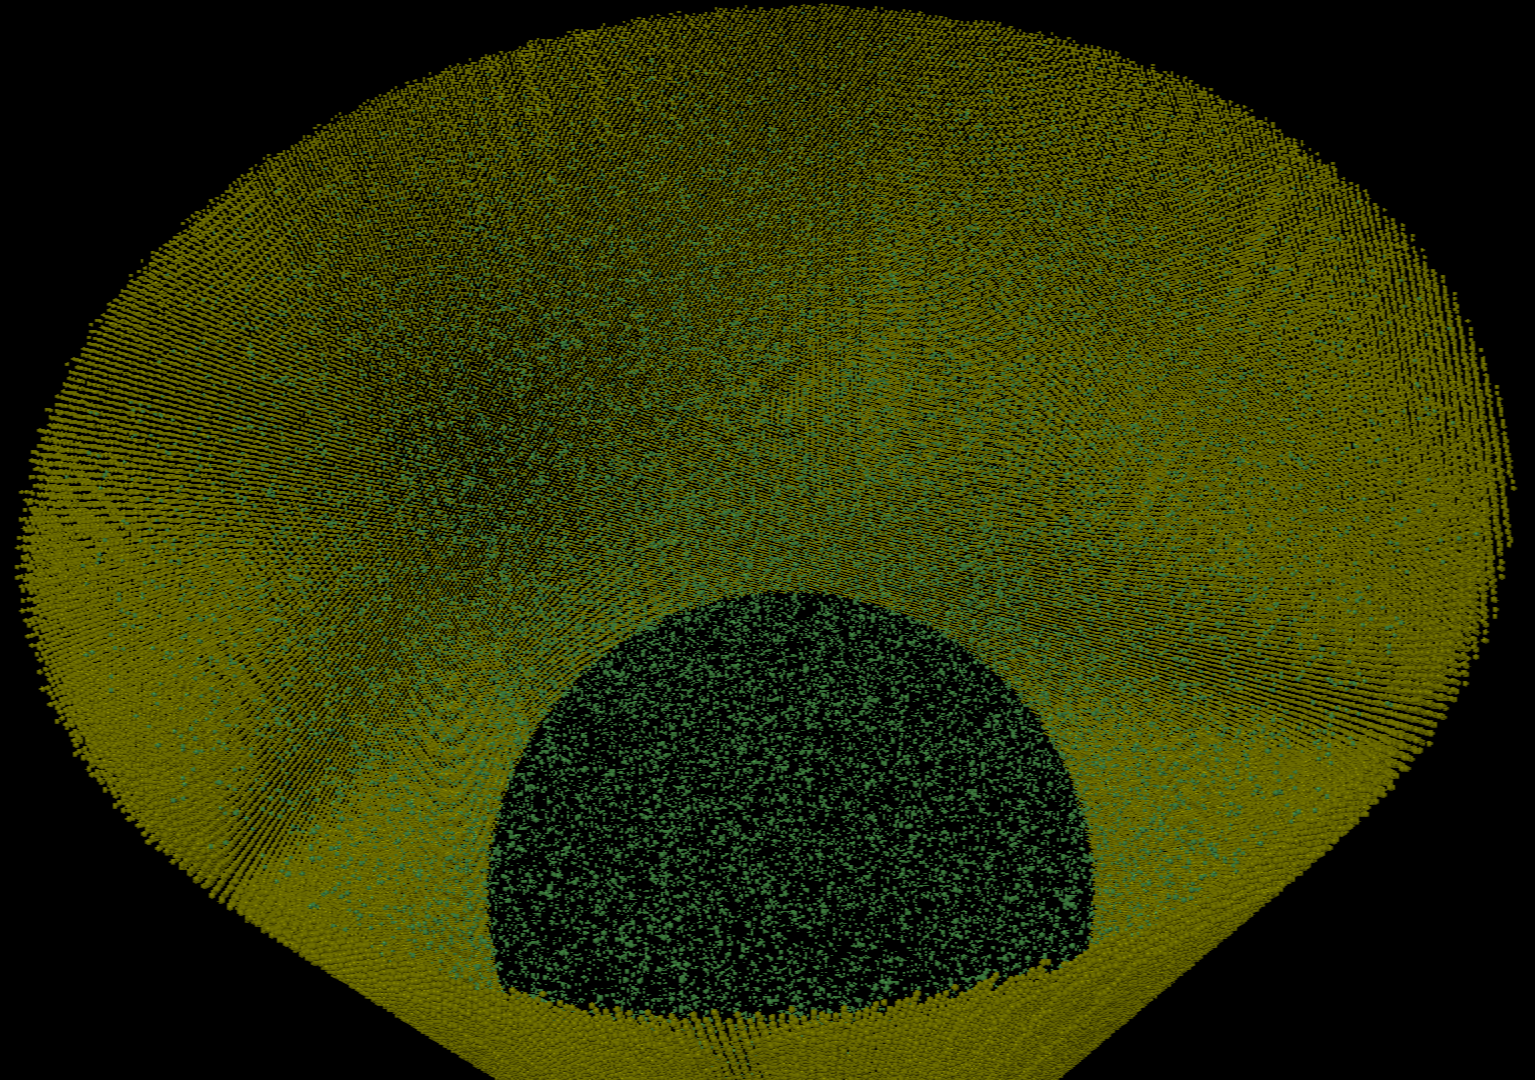
\includegraphics[width=0.8\textwidth, trim=0cm 0cm 0cm 0cm, clip]{MD/figures/md_cylinder.png}
\end{center}
\caption{The final cylinder we used to simulate gas to validate the Knudsen correction factor for the permeability (see section \ref{sec:knudsen_correction}). Here the yellow atoms are the solid wall (with a harmonic oscillator potential on each atom, keeping the atoms in place), and the green atoms are the gas. Since we have used a cut-off radius $r_\text{cut}=2.5\sigma$, we have removed the solid atoms outside the radius $r+2.5\sigma$. This visualization is done with the tool discussed and developed in chapter \ref{chap:particle_visualizer}.}
\label{fig:md_cylinder}
\end{figure}
Once we have the cylinder, we can choose the density yielding a desired Knudsen number
\begin{align}
	\rho_n(\text{Kn}) = \frac{1}{\sqrt 2 \pi d^2 \text{Kn}L},
\end{align}
where we have used $d=$\unit{3.62}{\angstrom} as we did in DSMC. The flow is induced in the same way as we did in DSMC (explained in section \ref{sec:dsmc_pressure}), where we can, given a pressure difference $\Delta P$, accelerate the atoms inside the cylinder according to equation \eqref{eq:acceleration_to_pressure_difference}
\begin{align*}
	g = \frac{\Delta P}{\rho_m\Delta x}.
\end{align*}
Here, $\Delta x$ is the system length in the flow direction, $L_z$. We have chosen a pressure difference equal to $0.2P_0$, where $P_0=\rho_nk_BT$ being the ideal gas pressure. We can then for each Knudsen number induce flow and measure the permeability. The system reached an equilibrium state before we sampled for $500000$ timesteps. In figure \ref{fig:md_permeability}, we have plotted the measured permeabilities for different Knudsen numbers with the Knudsen corrected analytical solution
\begin{align}
	\label{eq:cylinder_knudsen_corrected}
	k_a = [1 + \alpha(\text{Kn})\text{Kn}]\left[1 + {4\text{Kn}\over 1 + \text{Kn}}\right] {r^2\over 8}.
\end{align}
The left figure, using a logarithmic $x$-axis shows that the permeabilities in the lower range of the Knudsen numbers are predicted very by the theory. The right figure shows that the permeabilities in the whole range, two orders of magnitues, follows the expression in equation \eqref{eq:cylinder_knudsen_corrected}. For the high Knudsen numbers, we see an increase in the statistical noise which is explained by the fact that a high Knudsen number is obtained by a low density which gives a low number of atoms. In order to get better statistics, we would need to run the simulation for a longer time.
\begin{figure}[h]
\begin{center}
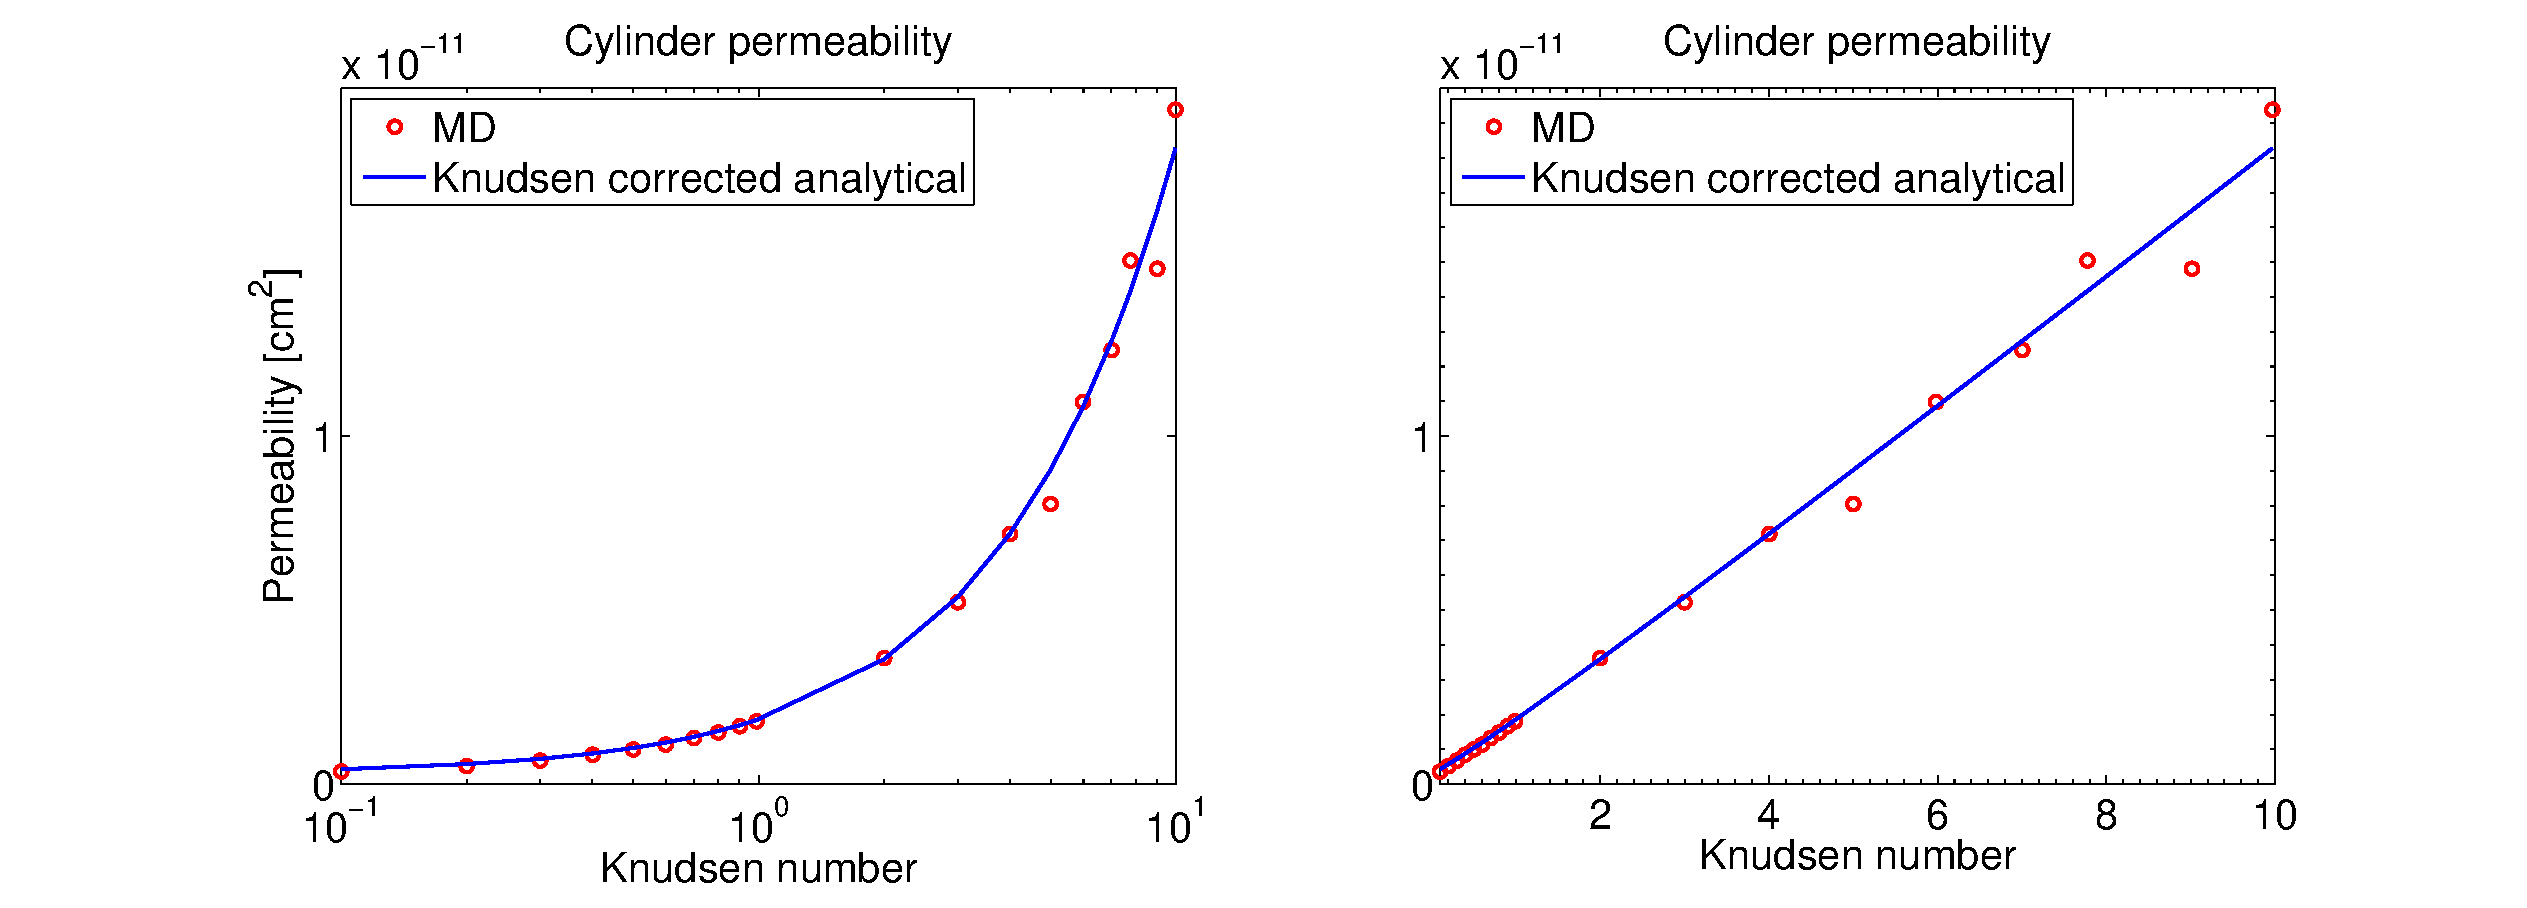
\includegraphics[width=1.0\textwidth, trim=0cm 0cm 0cm 0cm, clip]{MD/figures/permeability_cylinder.eps}
\end{center}
\caption{Permeabilities for Knudsen numbers in the range $0.1$ to $10.0$ in a cylinder with radius $r=$\unit{151}{\angstrom}. The left figure has a logarithmic $x-$axis to emphasize the good prediction in the lower Knudsen range. The right figure shows that the MD code produces results according to the Knudsen corrected permeability for a cylinder in equation \eqref{eq:cylinder_knudsen_corrected} in the entire range. The increased statistical noise is explained by that for large Knudsen numbers, the number of gas atoms is low.}
\label{fig:md_permeability}
\end{figure}